\documentclass[a4paper, 12pt]{scrartcl}
\usepackage[utf8]{inputenc}
\usepackage[T1]{fontenc}
\usepackage{lmodern}
\usepackage{graphicx} % support the \includegraphics command and options
\usepackage{subfig} % for subfloats
\usepackage{booktabs} % for tables
\usepackage{multirow} % for awesome tables
\usepackage{amsfonts}

\usepackage{varioref}
\usepackage{cleveref}
\usepackage{microtype} % Include and forget
\date{\today}
\title{Professional development}
\subtitle{Bouldering Wall}
\author{A. Dhar, J. Schloss, L. Li, V. Churavy}
\begin{document}
\maketitle
\paragraph{Introduction}
Our project will concern itself with planning and building a bouldering wall for the OIST family.
Bouldering as a sport has seen a uptake of interest in recent years across Europe and North America, leading to the creation of bouldering gyms in cities and at Universities. 

Bouldering is a form of sport climbing close to the ground and without the need of being belayed or wearing safety equipment like a harness, While bouldering the climber needs to focus on his balance on the wall, have the power and endurance to perform the next move, as well as a high degree of body control and foresight in planning his route. Being a good climber does not mean being the strongest or fastest but rather being efficient and elegant. This mentality attracts a diverse set of people to the sport and is one of the main reasons for its rise in popularity.

A bouldering wall normally consists of several pieces of wood with different degrees of inclination on which the climbing holds are fixed. To limit the dangers related to falling the floor of the wall needs to be covered with foam.

\paragraph{Construction of the Wall}
The wall itself consists of 12mm thick plywood that is reinforced by a frame made of wooden struts to carry the weight of the climber and to prevent flexing of the wood. The frame is the securely mounted to the base wall of the building. 
The foam mattress consists of a bottom layer of 20cm thick open foam and a top layer of 5cm closed foam, covered by a PVC sheet to protect the foam.
The two layer is necessary to prevent two distinct dangers that occur while climbing. The one is falling backwards of the wall and hurting you back and head in the process. The open foam layer is designed to absorb the force of the impact. The second danger is falling from the wall and landing on your feet. If the ground is too soft you might twist your ankle so the closed foam adds stability.
\Vref{wall1} shows a look at the back of the wall, with the supporting frames and trusses needed to hold the wall together and attach it to the I-beams. \Cref{wall2} shows how the wall will fit into the corner of the ceramics shed, with three I-beams as its main supports and the foam pads underneath.

\subparagraph{Fixing the frame to the building}
Also contingent on the exact location is the question how to fix the wall to building structure and what kind of modifications we can make to it.

To attach the wall to the building, we have designed the wall to line up with three I-beams in the corner of the ceramics shed. The wall will be fixed to each of these beams with a brace made from metal pipes and brackets. The metal tube can be attached to the wall using U bolts, and then placed around each I-beam at the top and bottom, anchoring the wall securely. This also makes it possible for the wall to be removable should the need arise.

\subparagraph{Making Holds}
The climbing holds should be made out of Polyurethane in a variety of different forms. To create these forms, we will first design them with florist foam and cover them with silicone to produce a mold. After placing the Polyurethane in the mold, we will place the entire structure in a vacuum chamber. The chamber will consist of a plastic bin with a single port at the top, where toxic fumes will be siphoned through a shop vacuum via its exhaust to a safe, removed location. This process is necessary for curing because gas bubbles in the plastic will result in structural weaknesses. 


\paragraph{Location and Access}
As location for the wall we currently propose the old clay factory in which the student wood workshop is also located, but this is contingent on the approval of the building management and also the exact placement of the wall inside the clay factory needs to be determined. We would prefer one of the corners to be more space efficient and fully utilize the foam mattress.

Special safety considerations must be taken into account if the bouldering wall is to be constructed next to the wood workshop. In particular, an internal organization should be created within OIST of individuals who wish to access the wall. Individuals in this organization should be briefed on basic safety for using the bouldering wall and being around the woodworking equipment, but do not need training in the usage of the equipment. Individuals who have not been trained in basic safety should not be granted access to the bouldering wall. To separate the bouldering wall and wood workshop, the space  between the wood workshop area and the bouldering wall should be separated by a line of a distracting color, such as red, green, or striped yellow and black. We must further discuss these plans with the members of the wood workshop to effectively utilize the shared space.



%TODO add info on access
\paragraph{Outreach}
Since none of us have specific experience in building rock climbing walls, we will be reaching out through the OIST community to acquire the expertise we require. Our first main contact is Julia Nabholz, who runs the Child Development Center. Her husband Mike is a construction worker and has offered us help in finding the right supplies to design our wall with. Julia will also be putting us in touch with another parent who has experience building rock climbing walls, and is currently designing one for the CDC's playground.

In addition, Michael Cooper and Maki Thomas have made us aware of a cafe owner who is interested in building a rock climbing wall at his cafe at the base of OIST, so while we will not be able to build this for him, we will meet with him to make sure our bouldering wall coexists with his rock climbing wall.

\paragraph{Materials}
For obtaining hardware and supplies, our main sources will be Tabata and Makeman. We will also try to take advantage of the workshop's supplies and tools when possible. With our current design and our preferred location we would need the parts listed in \cref{material}.

\subparagraph{Costs}
We visited Makeman at February 27th to get an estimate of the cost for the materials. The cost for the wood necessary for the whole wall is about $30000\yen$, divided into $17000\yen$ for the plywood sheeting and $13000\yen$ for the wooden struts. We estimate than we would need another $15000\yen$ for screws, metal pipes, brackets, wood-wood connectors and drill bits.
The second major cost point would be the safety mattress and we are currently exploring several options there.

The last cost point would be the holds. Commercial offering vary widely in price mostly depending on size. Medium size holds cost around $100\$$ for 15 pieces. On the other hand there are sets of holds available that consists of 100 holds in different sizes for about $200\$$. Casting our own holds would be cheaper, since we would only pay for the raw materials as well as allowing for more creative freedom. One litre of polyurethane resin costs abourt $15\$$

\newpage
\section*{Appendix}
\begin{figure}[ht]
\subfloat[View of frame and trusses to support the wall.]{
\label{wall1}
\centering
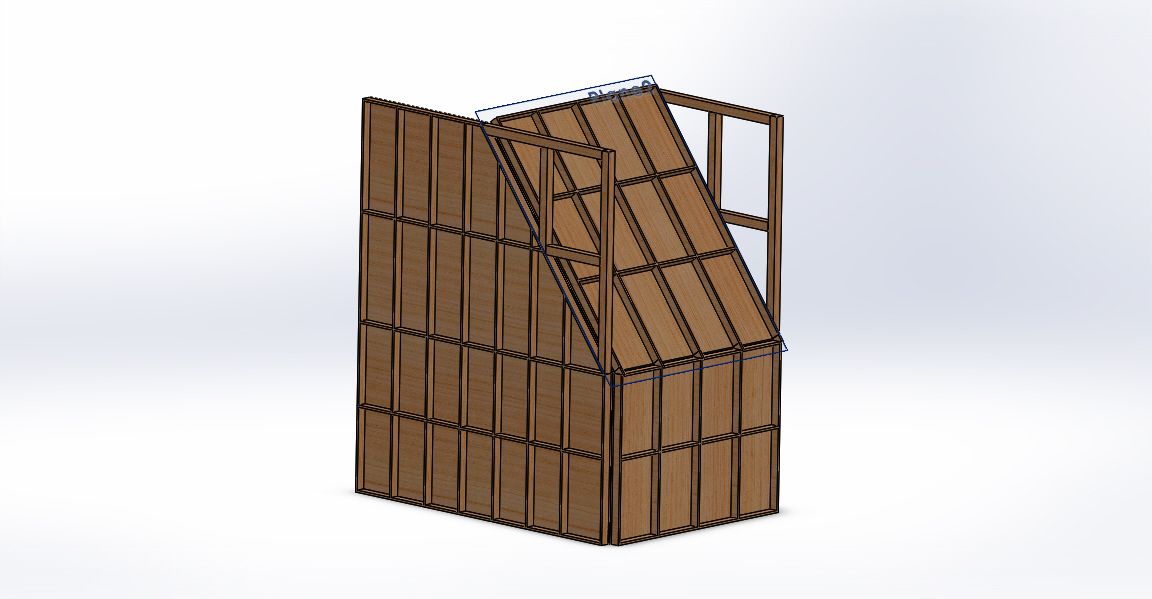
\includegraphics[width=.5\textwidth, clip=true, trim=200 0 200 0]{WoodWall2}
}
\subfloat[View of the rock climbing wall with respect to the building structure and I-beams.]{
\label{wall2}
\centering
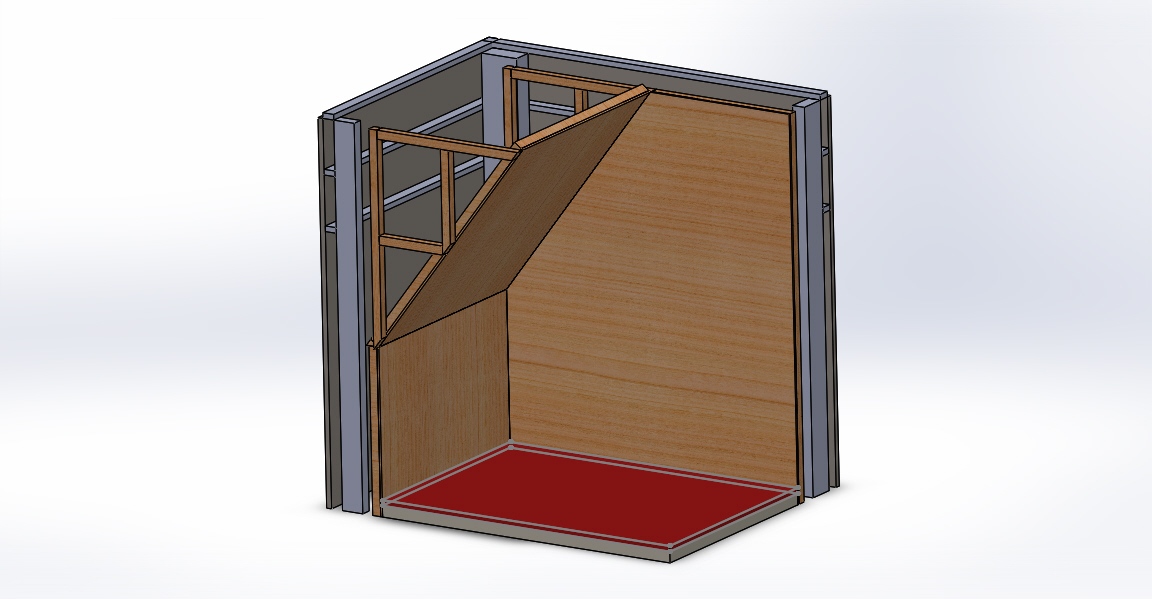
\includegraphics[width=.5\textwidth, clip=true, trim=200 0 200 0]{RockWall}
}
\end{figure}


\begin{table}[ht]
\centering
\caption{List of Materials}
\label{material}
\begin{tabular}{l l}
\toprule[2pt]
Section & Item\\
\midrule
\multirow{3}{*}{Frame} & 80m of 2x8cm struts \\
	& 10m of 8x8cm struts \\
	& Screws + connectors \\
\midrule
\multirow{2}{*}{Wall} & 16.5 $m^2$ of 12mm plywood (910x1820mm pieces)\\
	& T-nuts 500 [20cm grid] \\
\midrule
\multirow{3}{*}{Mattress} & 6$m^2$ of 5cm thick closed foam\\
	& 6$m^2$ of 10 cm thick open foam (ICD 58/IFD>=60)\\
	& $\approx$6$m^2$ pvc sheet\\
\midrule
\multirow{4}{*}{Holds} & Polyurethane resin\\
	& Florist foam\\
	& Silicone\\
	& 10 mm bolts\\
	\midrule
\multirow{2}{*}{Misc} &  Drill bits and bits\\
	& Tubing to connect to shop vac\\
\bottomrule[2pt]
\end{tabular}
\end{table}


\end{document}
